% Appendices are set up same as chapter sections
\chapter{Appendix - Interviews regarding baggage handling}

\section{Claude Monteils, Air France}
In order to understand what can happen to a wheelchair during this long period of time that includes transfer to the tarmac, loading in the cargo hold, and flight disturbances, we interviewed Claude Monteils, an Air France employee at Toulouse-Blagnac TLS Airport (France). Claude is responsible of the cargo hold management of the short range aircraft of Air France’s fleet at TLS and accepted to answer our questions about the way wheelchairs are handled and stored in the cargo hold.
\begin{figure}[h]
\centering

\includegraphics[width=4cm]{images/claude_monteils}
\caption{Claude Monteils - Air France employee at Toulouse airport (France)}
\label{fig:claude_monteils}
\end{figure}

\subsection{General procedure for wheelchair storage}
The type of wheelchair the passengers are equipped with really makes a difference in the way the airline will handle it:
\begin{easylist}[itemize]
& For a light wheelchair, that is to say a non powered wheelchair, the forces applied on the floor per square meter is very low. Therefore, these wheelchairs do not require any particular attention. They have the same status as a piece of luggage and are taken from the jet way to a conveyor belt that puts them into the cargo hold in the end so that once the aircraft has landed the wheelchairs are the first things that come out of the cargo hold. There is no box or protection or anything to protect this type of wheelchairs.
& For a heavy wheelchair (mostly powered wheelchairs), the problem is very different. First the wheelchair has to be able to enter the cargo hold (smaller than the door which is always the case for A320, B737 and bigger planes but Claude was not able to confirm this on smaller Embraer jets). Depending on the weight of the wheelchair, the force per square meter can be higher than what the cargo hold floor can stand. Since the contact area between the floor and the wheelchair is small (see\ref{fig:wheelchair_contact_area}) but the weight is high, it causes lots of issues. The only way for Air France passengers to make sure their heavy powered wheelchair can go to the cargo hold and be protected from all sorts of damage is to follow a very specific and long procedure.
\end{easylist}
\begin{figure}[h]
\centering
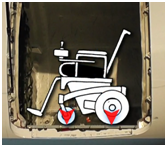
\includegraphics[width=7cm]{images/wheelchair_contact_area}
\caption{Contact area between the wheelchair and the cargo hold floor: its causes an important stress on the aircraft structure}
\label{fig:wheelchair_contact_area}
\end{figure}

\subsection{Specific procedure for heavy powered wheelchair which are stored in the cargo hold}
First, they have to tell Air France in advance that they are travelling with a heavy powered wheelchair and they have to give all the characteristics of their chair in advance. Usually, once they initiate the procedure, an Air France employee has to contact them to ask for more information and details.
The problem is that most of the time disabled passengers with powered wheelchairs do not mention it at all until check in or even boarding and when the airline finds out that they have to deal with a heavier than what the cargo hold floor can stand powered wheelchair, most of the time because they are afraid of being sued for denying a reduced mobility passenger the right to have his/her wheelchair in the cargo hold, they have to find a solution in a hurry and most of the time it’s not an optimal solution. They systematically use a sort of fake floor or wooden plates to distribute the load of the wheelchair and thus decrease the number of Newtons per square meters, even if the wheelchair happen to be light enough because they don’t have time to analyze it. In order to make sure the wheelchair will remain on this support they use ropes to tie it and they usually store it in a section of the cargo hold that is not dedicated to containers. The reason for it is that most of the time in such sections you have several nets to deter the objects from sliding and bumping (where as in the container compartment everything is already enclosed in boxes so no need to use nets).
However, when disabled passengers told in advance the airline about their powered wheelchair and sent in advance all the information to handle properly the wheelchair, things happens in a much better way. The personnel in charge of the cargo hold management can analyze whether the chair will require a fake floor to distribute its load or not, if so they usually try to adapt a container to shelter the wheelchair. As a consequence, when passengers leave their wheelchair at the jet way, the wheelchair directly goes to an adapted container and usually the airline employees use a lift instead of a conveyor belt to put the container in the cargo hold. The only inconvenience is that it’s a little bit longer to bring the wheelchair back to his/her owner once the plane has arrived at destination.

\subsection{Impacts on the center of gravity of the plane due to the presence of a heavy wheelchair in the cargo hold}
Before putting a wheelchair in the cargo hold the person in charge of the position of the center of gravity is notified the weight of the wheelchair (there is a weight measurement of everything that goes on a conveyor belt on a lift used for containers). Knowing the weight they use a computer to determine the best position for the wheelchair inside the cargo hold in order to make sure the center of gravity of the plane will remain stable during the flight.

However, it is necessary to have several powered wheelchairs on board (e.g. a team of handicapped athletes travelling altogether for a competition) to have a significant impact on the center of gravity of the plane, but in this case the airline generally knows a long time before the flight that they will have to deal with several power wheelchairs and they arrange everything in advance.
Once the wheelchair is on board the pilot is notified with the following information: the type of battery, in which compartment the chair was stored (front or rear, left or right), how heavy it is, etc. Since the pilot knows the chair is on board, why not the passenger? In fact nobody thinks about reassuring the passenger about his/her wheelchair, but it could be a good thing to do.

\subsection{Responsibilities of the airline employees}
In terms of responsibilities the airline employees have regarding wheelchair storage in the cargo hold, if the storage is arranged in advance there are several check-in points where each employee has to sign a document to testify that all the safety rules are respected so if something gets broken they are able to tell where and why. Most of the time for Air France when storage is arranged in advance, the wheelchairs are not damaged. If they are damaged it often happens in the cargo hold itself where no human operator can control it, but it’s rare. 
However, when storage is not arranged in advance, or when disabled people only have a non powered wheelchair that is considered as a piece of luggage, there are no check-in points during the whole storage process. There are surveillance cameras on the tarmac for safety reasons but most of the time the plane, catering, fuel truck, etc… hide the employees and they are free to do whatever they want with the wheelchair. If they break it nobody will blame them since nobody will know.

\section{Brandon Witta, Delta Airlines}
We were able to get in touch with Brandon Witta, a Ramp Agent for Delta Airlines at Hartsfield Jackson International Airport in Atlanta, Georgia. He answered a series of questions for us over email.

``All the information below is of the Atlanta operation. Each station has a similar operation but what makes ATL so different is the heavy flight schedule. I don't know the flights per day in ATL but I do know that Hartsfield-Jackson has been the busiest airport in the world since 2000. "

\begin{itemize}
\item What are the biggest constraints in the job? What are you most concerned about?

``Since the operation moves so quickly I think time is the biggest constraint.  The size of the operation also makes communication key amounst the ground crews, dispatch, and towers. Here are some other constraints; flights changing gates, on the ground gate changes, destination changes, bags missing flights, connecting bags to their connecting flights, travel times, unload times, loading times, \# of handlers per gate, \# of drivers per offload....I was in a meeting with one of the station managers last week and one concern he is focusing on this year was minimizing the number of bags missing their connecting flights, since more people are flying delta now more than ever it's hard to compinsate using the same staffing. He is focusing on connecting flights 35-45 minutes out. We run into problems during the offload since it takes 10-30 minutes to offload depending on the number of bags and type of aircraft. Anyways..note that electrical wheel chairs are never transported on the bag tugs, they are gate checked and given back to the customer upon arrival..however standard wheelchairs are commonly checked luggage and can be transported via tug."

\item What type of information (if any) do you get about specific wheelchairs before you handle them?

``The only information we get is the weight, which gives us an idea if it's a standard or an electrical wheelchair. Standard wheelchairs as well as electrical wheelchairs have similar designs so we handle them both the same."

\item How do you receive the information?

``Everything loaded on the plane is scanned and uploaded to a ramp worksheet that we process before a plane departs and arrives. It shows all the details of weight and balance. For example; \# of bags and their position, pounds of freight, valet bags, wheel chairs, strollers, live animals, dangerous goods, dry ice, and total pounds in each bin."

\item How would you like to receive the information? How can it be improved?

``Recieving the ramp worksheet is simple. "

\item How long would you spend handling a wheelchair? How long does it take?

``Typically a standard manual wheelchair takes 3 to 5 minutes to get to the jet bridge after a plane is parked. However electrical wheelchairs could take up to 10 minutes since some weigh up to 600 pounds! If they are too heavy to handle we use the elevator for transportation. "

\item How many handlers typically handle a wheelchair? How is information shared between them? 

``1 handler per standard wheelchair since they are light. For electrical wheelchairs there are 2 to 4 handlers depending how heavy it is."

\item  Is there a specific training module for handling wheelchairs? 

``Yes. We have annual training that covers the loading procedures for every piece that can possibly be loaded. This training covers lifting techniques to protect us from injury."

\item What kind of device is used to move a wheelchair from the jetway to the cargo hold?

``We typically use the closest elevator to the gate if the wheelchair is too heavy, which we do a lot. If not, we carry it up to the jet way or down to the bin, might take 3 to 10 minutes. But since disabled passengers are the first ones on the airplane and last ones off the airplane, their wheelchairs should be handled properly."

\item What would improve your luggage handling techniques (e.g. better tools, instructions, more time, etc.)?

``TIME and more staffing would definitely make things less stressful."
 
\end{itemize}